\chapter{MCMC Mixing for BCC Model on ENCODE Dataset} \label{app-mcmc-mixing-chapter}
In this appendix, we gather together all the MCMC draws to assess the mixing of the Markov Chain when applying the BCC model to the ENCODE datasets. The total number of clusters K is set to 3, and we consider $T=20,000$ MCMC total iterations where the first $5,000$ iterations are discarded for the burn-in period. In general, the algorithm seems to mix well and converges rapidly to the target posterior distribution. \emph{Figure \ref{mix-alpha-pic}} shows the trace-plot for the adherence parameters $\alpha_{m}$ for the Gene Expression (GE) and Methylation (ME) data sources. The expected values are $\hat{\alpha} = 0.89$ for ME and $\hat{\alpha} = 0.48$ for GE. \emph{Figure \ref{mix-pi-pic}} shows the trace-plot for the mixing proportions $\pi_{k}$ for each cluster $k=1,2,3$. The expected values are $\hat{\pi}_{1}=0.6$, $\hat{\pi}_{2}=0.12$ and $\hat{\pi}_{3}=0.28$. \emph{Figure \ref{mix-lambda-pic}} shows the trace-plot for the mean and variance parameter $\lambda_{k}$ of the Poisson mixture model for the K562 cell line. The expected values are $\hat{\lambda}_{1}=518$, $\hat{\lambda}_{2}=51$ and $\hat{\lambda}_{3}=273$. \emph{Figure \ref{mix-lambda2-pic}} shows the trace-plot for the mean and variance parameter $\lambda_{k}$ of the Poisson mixture model for the H1-hESC cell line. The expected values are $\hat{\lambda}_{1}=511$, $\hat{\lambda}_{2}=187$ and $\hat{\lambda}_{3}=261$. \emph{Figure \ref{mix-bin-pic}} shows the trace-plot for the probability of success parameter $\rho_{k}$ of the Binomial mixture model for the K562 cell line. The expected values are $\hat{\rho}_{1}=0.07$, $\hat{\rho}_{2}=0.74$ and $\hat{\rho}_{3}=0.28$. And finally, \emph{Figure \ref{mix-bin-pic}} shows the trace-plot for the probability of success parameter $\rho_{k}$ of the Binomial mixture model for the H1-hESC cell line. The expected values are $\hat{\rho}_{1}=0.04$, $\hat{\rho}_{2}=0.09$ and $\hat{\rho}_{3}=0.14$.

\begin{figure}[!ht]
\begin{center}
 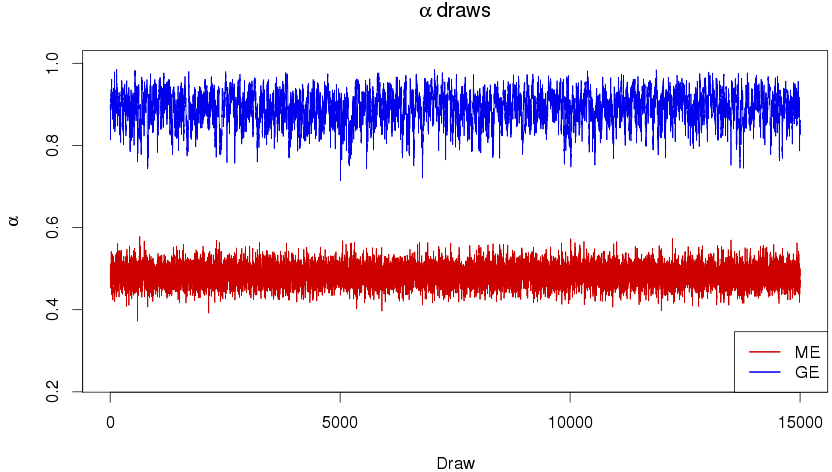
\includegraphics[scale = 0.63]{images/bccMV2DAlpha}
\caption{\emph{Trace-plot of the adherence parameter $\alpha_{m}$ for each data source Gene Expression (GE) and Methylation (ME) over the $15,000$ MCMC draws.}}
\label{mix-alpha-pic}
\end{center}
\end{figure}

\begin{figure}[!ht]
\begin{center}
 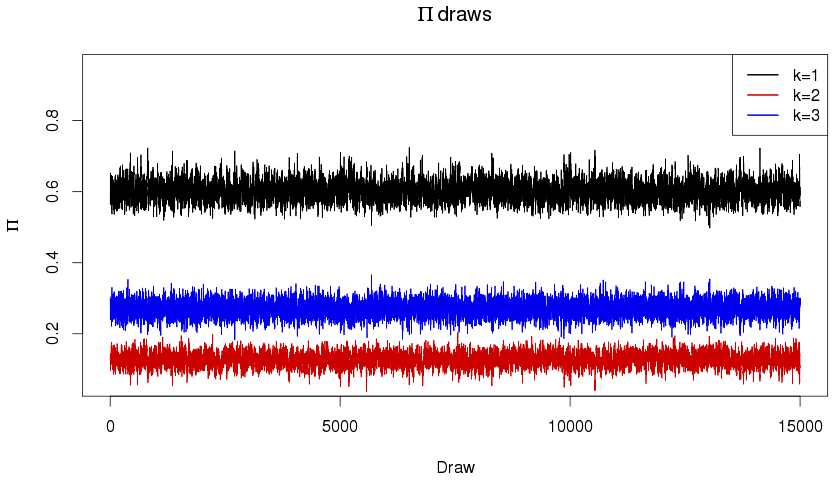
\includegraphics[scale = 0.63]{images/bccMV2DMixProp}
\caption{\emph{Trace-plot of the mixing proportions $\pi_{k}$ for each cluster $k=1,2,3$ over the $15,000$ MCMC draws.}}
\label{mix-pi-pic}
\end{center}
\end{figure}

\begin{figure}[!ht]
\begin{center}
 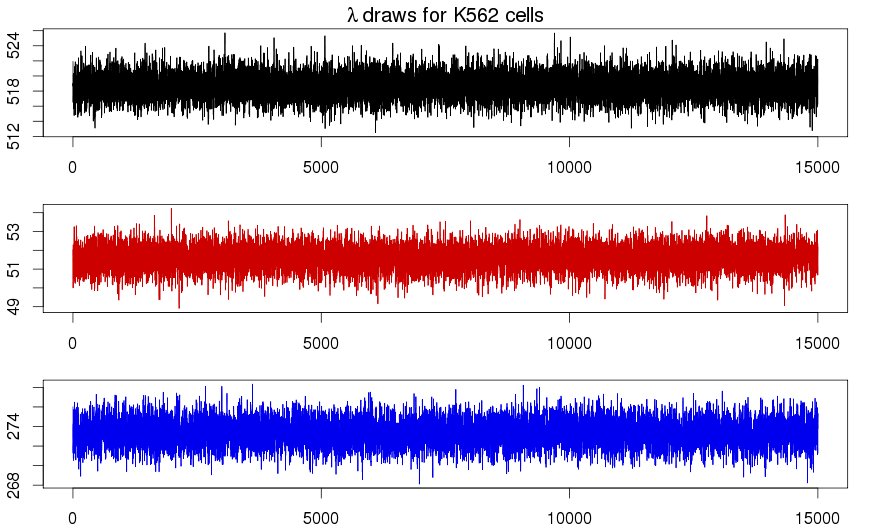
\includegraphics[scale = 0.46]{images/bccMV2DLambdak562}
\caption{\emph{Trace-plot of the $\lambda_{k}$ parameters of the Poisson mixture model for K562 cell line, for each cluster $k=1,2,3$ over the $15,000$ MCMC draws.}}
\label{mix-lambda-pic}
\end{center}
\end{figure}

\begin{figure}[!ht]
\begin{center}
 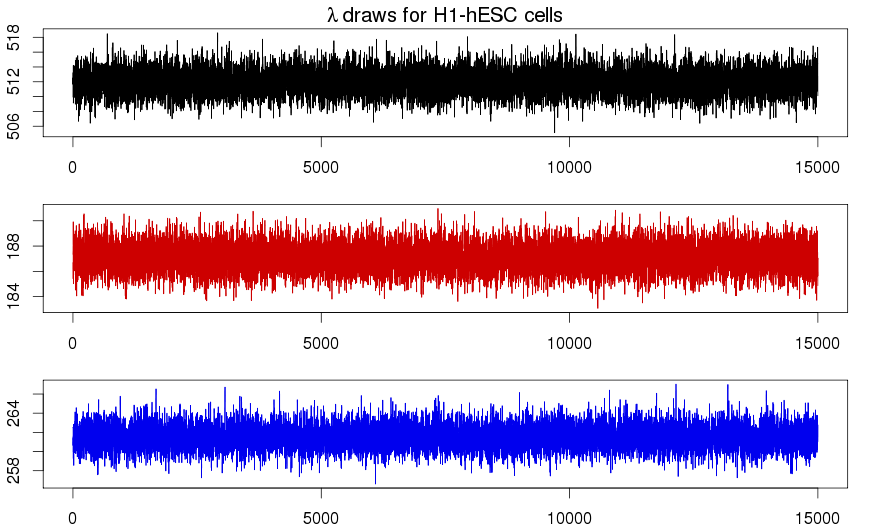
\includegraphics[scale = 0.46]{images/bccMV2DLambdah1}
\caption{\emph{Trace-plot of the $\lambda_{k}$ parameters of the Poisson mixture model for H1-hESC cell line, for each cluster $k=1,2,3$ over the $15,000$ MCMC draws..}}
\label{mix-lambda2-pic}
\end{center}
\end{figure}


\begin{figure}[!ht]
\begin{center}
 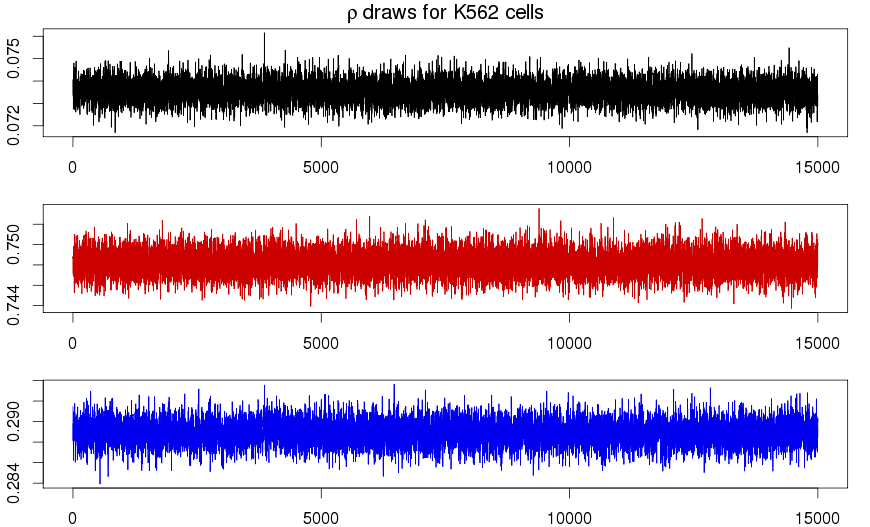
\includegraphics[scale = 0.46]{images/bccMV2DBinomk562}
\caption{\emph{Trace-plot of the $\rho_{k}$ parameters of the Binomial mixture model for K562 cell line, for each cluster $k=1,2,3$ over the $15,000$ MCMC draws..}}
\label{mix-bin-pic}
\end{center}
\end{figure}

\begin{figure}[!ht]
\begin{center}
 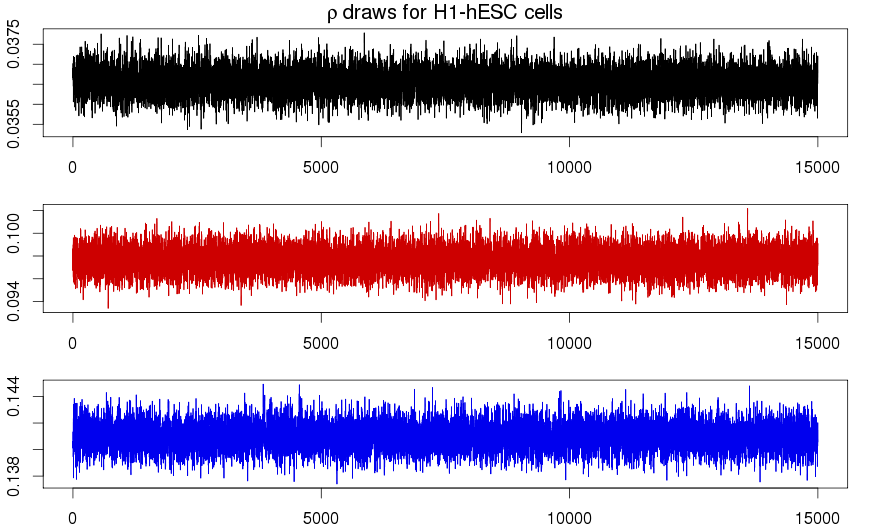
\includegraphics[scale = 0.46]{images/bccMV2DBinomh1}
\caption{\emph{Trace-plot of the $\rho_{k}$ parameters of the Binomial mixture model for H1-hESC cell line, for each cluster $k=1,2,3$ over the $15,000$ MCMC draws..}}
\label{mix-bin2-pic}
\end{center}
\end{figure}